\documentclass[aspectratio=169,11pt]{beamer}
\usepackage{presentation-theme}
\hypersetup{pdftitle={Encoder chemistry: token-level and mechanistic checkpoint comparison},pdfauthor={Wuhao},pdfsubject={Native JAX checkpoint study, 30 September 2026}}
\newcommand{\bodytext}[4]{\node[anchor=north west,inner sep=0,align=left,text width=#3cm,font=\figurefont\fontsize{10}{13}\selectfont] at (#1,#2) {#4};}
\newcommand{\plotfigure}[1]{\node[anchor=north,inner sep=0] at (8,6.78) {\includegraphics[width=14.3cm,height=4.75cm,keepaspectratio]{figures/#1_slide.pdf}};}
\newcommand{\studydata}{MassSpecGym 1.5: 4,096 / 1,024 / 1,024 train / validation / test molecular connectivities. Frozen native JAX encoders.}
\newcommand{\probepolicy}{Physical peak tokens; CLS excluded. Three readout seeds; learning rate and epoch selected on validation.}
\newcommand{\saepolicy}{Raw block 19; 8,192 SAE features; train-only normalization; equal molecule weight. No chemistry labels enter SAE training.}
\begin{document}

% 01: A measured conclusion, with the pooling question answered directly.
\begin{frame}
\begin{tikzpicture}[remember picture,overlay,shift={(current page.south west)}]
\header{ENCODER CHEMISTRY / 30 SEP 2026}{}
\node[anchor=north west,inner sep=0,font=\brandmedium\fontsize{25}{29}\selectfont,text width=13.8cm,align=left] at (.75,7.25) {Does latent training improve\\token-level chemical meaning?};
\bodytext{.85}{5.05}{13.8}{\textbf{Token-aware chemical readouts favor the parent.}\\The latest checkpoint is easier to reconstruct sparsely and more resistant to peak removal, but neither establishes better chemical alignment.}
\node[anchor=north west,inner sep=0,font=\brandmedium\fontsize{31}{35}\selectfont] at (.85,3.5) {0.7987\quad$\rightarrow$\quad0.7750};
\bodytext{.85}{2.4}{13.8}{Final-token MACCS AUROC: parent 1,190k / periodic student 1,209k}
\takeaway{Attention helps both encoders; sparse autoencoders and causal tests refine what the difference means.}
\source{Native JAX checkpoint comparison. 1,024 held-out molecules; ensemble of three token-attention readouts. Parent initializes the periodic teacher, not the student.}
\end{tikzpicture}
\end{frame}

% 02
\begin{frame}
\begin{tikzpicture}[remember picture,overlay,shift={(current page.south west)}]
\header{01 / CHECKPOINT LINEAGE}{These checkpoints come from different training histories}
\plotfigure{checkpoint_lineage}
\takeaway{The periodic student starts fresh; this is not 19,000 further updates of the parent encoder.}
\source{Pinned latest committed checkpoint: 1,209,000. Parent: 1,190,000; stored periodic teacher: 1,200,000. Teacher copies every 50,000 updates. No matched nonpromotion control was run.}
\end{tikzpicture}
\end{frame}

% 03
\begin{frame}
\begin{tikzpicture}[remember picture,overlay,shift={(current page.south west)}]
\header{02 / EXPERIMENTAL DESIGN}{Separate feature discovery from held-out evaluation}
\foreach \x/\title/\count in {1.0/Train/{4,096},6.0/Validation/{1,024},11.0/Test/{1,024}}{
 \node[anchor=north west,inner sep=0,font=\brandmedium\fontsize{17}{20}\selectfont] at (\x,6.55) {\title};
 \node[anchor=north west,inner sep=0,font=\brandmedium\fontsize{25}{28}\selectfont] at (\x,5.55) {\count};
}
\draw[line] (5.35,2.55)--(5.35,6.6);\draw[line] (10.35,2.55)--(10.35,6.6);
\bodytext{1.0}{4.15}{3.8}{Fit readouts\\Train SAEs\\Fit normalization\\Align replicas}
\bodytext{6.0}{4.15}{3.8}{Tune readouts\\Freeze features\\Select layers\\Set thresholds}
\bodytext{11.0}{4.15}{3.8}{Score chemistry\\Run interventions\\Check controls\\Keep failures}
\takeaway{One representative spectrum per connectivity identity; all candidate choices precede test evaluation.}
\source{\studydata\ 166 MACCS bits, seven elements, 15 SMARTS functional groups. Highest-activation example cards are separately labeled post-confirmation illustrations.}
\end{tikzpicture}
\end{frame}

% 04
\begin{frame}
\begin{tikzpicture}[remember picture,overlay,shift={(current page.south west)}]
\header{03 / TOKEN-AWARE CHEMISTRY}{Learned token attention does not reverse the parent advantage}
\plotfigure{token_attention}
\takeaway{Latest block-19 attention gains 0.0052 MACCS AUROC over mean pooling; the parent remains stronger.}
\source{\probepolicy\ AUROC of mean seed logits; 1,024 test molecules. 145 MACCS and 13 functional-group targets with shared support. Paired molecule bootstrap, descriptive 95\% intervals.}
\end{tikzpicture}
\end{frame}

% 05
\begin{frame}
\begin{tikzpicture}[remember picture,overlay,shift={(current page.south west)}]
\header{04 / LAYER AND TOKEN GEOMETRY}{Representation shape changes with depth and normalization}
\plotfigure{token_geometry}
\takeaway{A low-rank layer and a high-rank final output can coexist; rank alone does not measure chemical meaning.}
\source{Geometry at eight selected states across all 6,144 panel molecules; rank uses a fixed 256-dimensional projection. Held-out input decoding. N: final RMSNorm; O: final affine output. Pooled chemical probes cover all 28 states.}
\end{tikzpicture}
\end{frame}

% 06
\begin{frame}
\begin{tikzpicture}[remember picture,overlay,shift={(current page.south west)}]
\header{05 / INTERPRETABILITY DESIGN}{Decompose token activations, then intervene in the native encoder}
\plotfigure{token_sae_interventions}
\takeaway{Feature removal preserves the reconstruction residual; controls use the same requested token amplitudes.}
\source{\saepolicy\ Half/full feature removal; firing-matched feature and orthogonal random directions. Three fixed final-token readouts. No positive steering or sufficiency test.}
\end{tikzpicture}
\end{frame}

% 07
\begin{frame}
\begin{tikzpicture}[remember picture,overlay,shift={(current page.south west)}]
\header{06 / SIX SPARSE AUTOENCODERS}{The latest token states are more sparsely reconstructable}
\plotfigure{sae_reconstruction}
\takeaway{At 32 active features per token, held-out variance explained rises from 72.8\% to 89.1\%.}
\source{\saepolicy\ Two seeds at k=32 and one k=64 control per encoder. 22,474 sampled test tokens with equal molecule weights. All selected fits reached the 40-epoch budget; convergence is not established.}
\end{tikzpicture}
\end{frame}

% 08
\begin{frame}
\begin{tikzpicture}[remember picture,overlay,shift={(current page.south west)}]
\header{07 / CHEMICAL FEATURE ASSOCIATIONS}{Useful halide features coexist with weak chemical candidates}
\plotfigure{chemical_features}
\takeaway{Ten candidates per encoder were frozen before test; the failed nitrile features remain in the analysis.}
\source{Two candidates each: amide, hydroxyl, halide, nitrile, sulfonyl. No amine candidate passed. Test AUROC uses molecular maximum feature activation; dense-channel and random-dictionary baselines are available.}
\end{tikzpicture}
\end{frame}

% 09
\begin{frame}
\begin{tikzpicture}[remember picture,overlay,shift={(current page.south west)}]
\header{08 / REPLICATION}{Stability is necessary evidence, but it does not guarantee chemistry}
\plotfigure{feature_stability}
\takeaway{Halide features replicate; stable activations can also encode acquisition or peak-count variation.}
\source{Train-only, label-free feature alignment; test activation Spearman. Each point averages two frozen features per concept. IDs are dictionary-local; two latest hydroxyl features share one replica.}
\end{tikzpicture}
\end{frame}

% 10
\begin{frame}
\begin{tikzpicture}[remember picture,overlay,shift={(current page.south west)}]
\header{09 / CAUSAL FEATURE EFFECTS}{Selected sparse directions influence the chemical readouts}
\plotfigure{sae_causal}
\takeaway{38 of 40 full-dose feature-versus-control contrasts pass Holm correction; chemical specificity is weaker.}
\source{512 independent test molecules. Mean logit shifts across three fixed readouts. 20 frozen features $\times$ two controls; paired t approximations with Holm correction. Bootstrap intervals are descriptive.}
\end{tikzpicture}
\end{frame}

% 11
\begin{frame}
\begin{tikzpicture}[remember picture,overlay,shift={(current page.south west)}]
\header{10 / A NECESSARY DISTINCTION}{Causal readout influence can coexist with failed recognition}
\node[anchor=north west,inner sep=0,font=\brandmedium\fontsize{16}{19}\selectfont] at (1.0,6.5) {Latest nitrile feature f3348};
\bodytext{1.0}{5.48}{6.1}{Held-out chemical association\\\textbf{AUROC 0.496}\\\vspace{4mm}Full feature removal\\\textbf{Nitrile-logit change $-0.0348$}}
\draw[line] (7.7,2.4)--(7.7,6.55);
\node[anchor=north west,inner sep=0,font=\brandmedium\fontsize{16}{19}\selectfont] at (8.3,6.5) {Reconstruction damage};
\bodytext{8.3}{5.48}{6.0}{Full SAE reconstruction:\\Balanced BCE increase\\\textbf{Parent $+0.01145$}\\\textbf{Latest $+0.01312$}\\\vspace{3mm}Other labels and negative\\molecules also respond.}
\takeaway{A feature can drive a chemical prediction without reliably detecting that chemical group.}
\source{Association: 1,024 test molecules. Causal/reconstruction effects: 512 molecules; train- and test-supported targets. Latest f3348 is a prespecified failed candidate, retained without reselection.}
\end{tikzpicture}
\end{frame}

% 12
\begin{frame}
\begin{tikzpicture}[remember picture,overlay,shift={(current page.south west)}]
\header{11 / MOLECULAR CASE STUDY}{A replicated halide feature still has strong false positives}
\plotfigure{halide_case}
\takeaway{Chemical motifs label the molecule; activated peaks are not validated assignments to those motifs.}
\source{Latest raw-19 SAE feature f7363. Positive and false-positive examples follow the frozen atlas selection: highest test activation within each class, chosen after confirmation. Measured spectra; illustrative cases.}
\end{tikzpicture}
\end{frame}

% 13
\begin{frame}
\begin{tikzpicture}[remember picture,overlay,shift={(current page.south west)}]
\header{12 / CHEMICAL NEIGHBORS}{The full-bank decline weakens after nuisance matching}
\plotfigure{chemical_neighbors}
\takeaway{Within strict mass and acquisition controls, the checkpoint difference is inconclusive.}
\source{Test-to-train SAE-max cosine neighbors. Full: 1,024 queries; matched: 472 with at least two candidates. Same instrument/adduct/CE presence; 5 Da / 10 CE / 5-peak calipers. $\Delta$: latest minus parent.}
\end{tikzpicture}
\end{frame}

% 14
\begin{frame}
\begin{tikzpicture}[remember picture,overlay,shift={(current page.south west)}]
\header{13 / COMPONENT NECESSITY}{Branch effects and individual-head effects differ}
\plotfigure{component_heads}
\takeaway{The parent's block-23 head 6 has a strong effect; head contributions are not an additive decomposition.}
\source{All 25 attention/MLP/conditioning branches screened on 256 validation molecules. Three layers per branch frozen, then tested on 512 molecules; 24 heads per encoder. Test rankings are descriptive.}
\end{tikzpicture}
\end{frame}

% 15
\begin{frame}
\begin{tikzpicture}[remember picture,overlay,shift={(current page.south west)}]
\header{14 / ACTIVATION RESCUE}{Restoring corrupted peak states recovers the original output}
\plotfigure{activation_rescue}
\takeaway{Selected-token rescue beats random slots, but chemistry-loss recovery is inconclusive in this cohort.}
\source{256 test molecules; top-20\% peak intensities multiplied by 0.1. Curves show selected-minus-random recovery from clean-state patches at raw depths 0--25; equal slot counts. Full-state rescue is exactly clean.}
\end{tikzpicture}
\end{frame}

% 16
\begin{frame}
\begin{tikzpicture}[remember picture,overlay,shift={(current page.south west)}]
\header{15 / ROBUSTNESS}{Peak-removal damage decreases, while clean error remains higher}
\plotfigure{input_robustness}
\takeaway{Smaller corruption damage does not reverse the parent advantage in absolute chemical prediction.}
\source{1,024 test molecules; ordinary BCE averaged over 177 train-active outputs using mean sigmoid scores across readouts. Different from class-balanced causal BCE. Paired molecule intervals. * Artificial $m/z$ perturbations.}
\end{tikzpicture}
\end{frame}

% 17
\begin{frame}
\begin{tikzpicture}[remember picture,overlay,shift={(current page.south west)}]
\header{16 / METADATA PATHS}{Route observed collision energy through two separate paths}
\plotfigure{metadata_paths}
\takeaway{The same measured spectrum receives old or observed-repeat energy through block and final conditioning.}
\source{689 eligible same-molecule repeats. Raw block-25 patching separates upstream conditioning from the final affine path. All valid slots, including CLS, are patched. Both diagonal self-patches are exact.}
\end{tikzpicture}
\end{frame}

% 18
\begin{frame}
\begin{tikzpicture}[remember picture,overlay,shift={(current page.south west)}]
\header{17 / ACQUISITION SENSITIVITY}{The latest chemical readouts are more sensitive to collision energy}
\plotfigure{metadata_effects}
\takeaway{Near-zero average final-path loss change does not imply zero response in individual predictions.}
\source{Observed CE swap on 689 shared molecules. Ordinary BCE over 177 train-active outputs; paired molecule intervals. Path interaction includes nonlinear encoder/readout/loss effects. Repeat cosine is readout-logit cosine.}
\end{tikzpicture}
\end{frame}

% 19
\begin{frame}
\begin{tikzpicture}[remember picture,overlay,shift={(current page.south west)}]
\header{18 / EVIDENCE SYNTHESIS}{Compressibility, chemistry and robustness give different answers}
\node[anchor=north west,inner sep=0,font=\brandmedium\fontsize{13}{16}\selectfont] at (1.0,6.55) {Question};
\node[anchor=north west,inner sep=0,font=\brandmedium\fontsize{13}{16}\selectfont] at (7.65,6.55) {Latest versus parent};
\foreach \y/\left/\right in {5.65/{Token-attention chemistry}/{Parent stronger},4.87/{Sparse reconstruction}/{Latest stronger},4.09/{Matched chemical neighbors}/{Difference inconclusive},3.31/{Peak-removal robustness}/{Latest loses less, but starts worse},2.53/{Collision-energy invariance}/{Latest more sensitive}}{
 \bodytext{1.0}{\y}{6.0}{\left}
 \bodytext{7.65}{\y}{6.6}{\right}
 \draw[line,line width=.4pt] (1.0,\y-.49)--(14.55,\y-.49);
}
\takeaway{The evidence does not support an overall chemical-semantic improvement at this endpoint.}
\source{Checkpoint comparison conditional on the measured panel, readouts and interventions. These results do not isolate the causal effect of the training recipe or promotion schedule.}
\end{tikzpicture}
\end{frame}

% 20
\begin{frame}
\begin{tikzpicture}[remember picture,overlay,shift={(current page.south west)}]
\header{APPENDIX / NUMERICAL CONTRACT}{The interventions reproduce the actual cached encoder function}
\bodytext{1.0}{6.5}{6.2}{\textbf{Primary computation}\\Native JAX, BF16 residuals, H100, batch 8. Full encoder trace; readouts compiled separately.\\\vspace{3mm}\textbf{Exact checks}\\Both caches match native pilots bitwise. Identity patches and inactive-feature edits change no logits.}
\bodytext{8.15}{6.5}{6.1}{\textbf{Why execution details matter}\\Latest native batch 16 differs from batch 8 by 2.585\% relative L2. PyTorch execution also differs despite identical weights.\\\vspace{3mm}\textbf{Feature checks}\\19,390 physical-token codes per arm match exports exactly; realized BF16 control norms are only approximately matched.}
\takeaway{Archived batch-16 and older PyTorch results are excluded from this report's primary measurements.}
\source{Native pilot, extraction, precision diagnostic, causal manifests and sparse-code audit. No claim of exact TPU--H100 equivalence. Full requested feature/control norms match before BF16 casting.}
\end{tikzpicture}
\end{frame}

% 21
\begin{frame}
\begin{tikzpicture}[remember picture,overlay,shift={(current page.south west)}]
\header{APPENDIX / CLAIM BOUNDARIES}{A tested mechanism is narrower than a complete chemical circuit}
\bodytext{1.0}{6.5}{6.2}{\textbf{Established}\\Token-level chemical signal.\\Replicated sparse associations.\\Feature and component effects.\\Token rescue and metadata paths.}
\bodytext{1.0}{3.95}{6.2}{\textbf{Unresolved}\\Training-recipe causality.\\Pretraining overlap.\\Rare chemistry and generalization.}
\bodytext{8.15}{6.5}{6.1}{\textbf{Not demonstrated}\\Positive steering or sufficiency.\\Head-to-feature mediation.\\Validated peak/fragment links.\\An exhaustive chemical circuit.}
\bodytext{8.15}{3.95}{6.1}{\textbf{Next tests}\\Matched training controls.\\Independent chemistry data.\\Fragment labels and path mediation.}
\takeaway{Keep the parent as the chemistry reference and retain token-aware evaluation before claiming a gain.}
\source{One checkpoint per training history. Molecule-bootstrap uncertainty is conditional on fixed models; most secondary intervals are unadjusted. Highest-activation examples are illustrative, not new confirmation.}
\end{tikzpicture}
\end{frame}

% 22
\begin{frame}
\begin{tikzpicture}[remember picture,overlay,shift={(current page.south west)}]
\header{APPENDIX / SOURCES AND REPRODUCTION}{Figures and conclusions trace back to the completed study}
\bodytext{1.0}{6.5}{13.7}{\textbf{Study artifacts}\\\texttt{artifacts/encoder\_chemistry\_20260930/}\\Checkpoints, readouts, six SAEs, interventions, cases and independent audit.}
\bodytext{1.0}{4.75}{13.7}{\textbf{Editable report and rebuild}\\\texttt{presentations/encoder\_chemistry/encoder\_chemistry.tex}\\\texttt{bash presentations/encoder\_chemistry/build.sh}\\Vector figures, compact inputs and source bundle included.}
\node[anchor=north west,inner sep=0,align=left,text width=13.7cm,font=\figurefont\fontsize{9}{11}\selectfont] at (1.0,2.65) {\textbf{Methods:} Gao et al. (2024), SAEs; Zhang \& Nanda (2023), activation patching.\\Chanin et al. (2024), feature splitting and absorption.};
\takeaway{Every measured chart uses saved results; explanatory diagrams are labeled as computation or intervention.}
\source{\href{https://arxiv.org/abs/2406.04093}{arXiv:2406.04093}; \href{https://arxiv.org/abs/2309.16042}{arXiv:2309.16042}; \href{https://arxiv.org/abs/2409.14507}{arXiv:2409.14507}. Report date: 30 September 2026.}
\end{tikzpicture}
\end{frame}
\end{document}
